\taskpic{ Имеется бесконечная проволочная сетка с прямоугольной
  ячейкой. Сопротивление каждой из проволок, составляющих ячейку,
  равно $r$. Найдите сопротивление между двумя соседними точками. }
{
  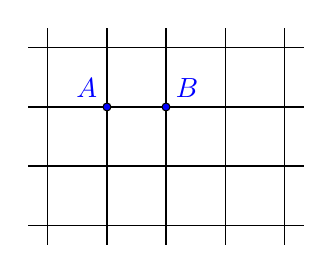
\begin{tikzpicture}
    \foreach \x in {0.5,1.25,2,2.75,3.5}
    \draw (\x,0) -- ++(0,2.75);
    \foreach \y in {0.5,1.25,2,2.75}
    \draw[yshift=-0.25cm] (0.25,\y) -- ++(3.5,0);
    \draw[fill=blue] (1.25,1.75) circle (0.05cm) node[blue,anchor=south east] {$A$};
    \draw[fill=blue] (2,1.75) circle (0.05cm) node[blue,anchor=south
    west] {$B$};
  \end{tikzpicture}
}